\section{Ilustrações}%
\label{sect:ill}

O pacote \texttt{utfpr-thesis} está configurado para definir ambientes para os seguintes tipos de ilustrações: figuras (\texttt{figure}), fluxogramas (\texttt{flowchart}), fotografias (\texttt{photograph}), gráficos (\texttt{graph}) e quadros (\texttt{tabframed}).
Exemplos de uso destes ambientes estão em arquivos-fonte deste modelo, conforme as \Cref{ssect:fig,ssect:fcht,ssect:phot,ssect:grph,ssect:tfrm}.

\subsection{Figuras}%
\label{ssect:fig}

Os ambientes \texttt{picture} (do \ifbool{MakeGly}{\gly*{LaTeX}}{\LaTeX}) e \texttt{tikzpicture}\footnote{Ver exemplos em \url{https://texample.net/}} (pacote \texttt{tikz}) permitem programar diversos tipos de ilustrações diretamente no \ifbool{MakeGly}{\gly*{LaTeX}}{\LaTeX}, como na \Cref{fig:ex-tikzpicture}.

\begin{figure}[!htbp]
\SetCaptionWidth{0.7\textwidth}
\begin{minipage}{\CaptionWidth}
\caption[%
  Primeiro exemplo de figura, produzida em ambiente \texttt{tikzpicture} a partir de arquivo-fonte: cone truncado%
]{%
  Primeiro exemplo de figura, produzida em ambiente \texttt{tikzpicture} a partir de arquivo-fonte\footnote{\texttt{fig-ex-tikzpicture.tex} em \texttt{./Chapter-Example/Illustrations/}.}: cone truncado%
}%
\label{fig:ex-tikzpicture}
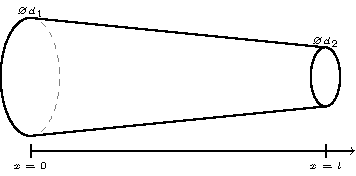
\includegraphics[width = \CaptionWidth]{fig-ex-tikzpicture}
\end{minipage}
\SourceOrNote{adaptada de \textcite{Magdowski2012}}
\end{figure}

Outros exemplos deste tipo de ilustração são apresentados nas \Cref{fig:subfig,fig:ex-uml}.

\subsubsection{Subfiguras}%
\label{sssect:subfig}

É possível produzir subfiguras e imprimir suas respectivas legendas a partir de comandos definidos na classe \texttt{\ifbool{MakeGly}{\gly*{memoir}}{memoir}}:

\begin{snugshade}
\begin{Verbatim}
\subtop[Subtitle\label{Label}]{Subfigure}%   % Acima da subfigura
\subbottom[Subtitle\label{Label}]{Subfigure}%% Abaixo da subfigura
\end{Verbatim}
\end{snugshade}

Além disso, é possível rotular e referenciar as mesmas, por exemplo, as \Cref{sfig:subfig-a,sfig:subfig-b,sfig:subfig-c,sfig:subfig-d,sfig:subfig-e} são exemplos de subfiguras da \Cref{fig:subfig}.

\begin{figure}[!htbp]
\SetCaptionWidth{\textwidth}
\caption{Segundo exemplo de figura, contendo cinco subfiguras}%
\label{fig:subfig}
\subbottom[Primeira subfigura\label{sfig:subfig-a}]{%
  \includegraphics[width = 0.3\CaptionWidth, page = 1]{example-movie}%
}%
\hspace*{0.05\CaptionWidth}%
\subbottom[Segunda subfigura\label{sfig:subfig-b}]{%
  \includegraphics[width = 0.3\CaptionWidth, page = 16]{example-movie}%
}%
\hspace*{0.05\CaptionWidth}%
\subbottom[Terceira subfigura\label{sfig:subfig-c}]{%
  \includegraphics[width = 0.3\CaptionWidth, page = 31]{example-movie}%
}%
\\%
\subbottom[Quarta subfigura\label{sfig:subfig-d}]{%
  \includegraphics[width = 0.3\CaptionWidth, page = 46]{example-movie}%
}%
\hspace*{0.05\CaptionWidth}%
\subbottom[Quinta subfigura\label{sfig:subfig-e}]{%
  \includegraphics[width = 0.3\CaptionWidth, page = 61]{example-movie}%
}%
\SourceOrNote{\textcite{Scharrer2018}}
\end{figure}

Sublegendas do tipo \labelcref{sfig:subfig-a,sfig:subfig-b,sfig:subfig-c,sfig:subfig-d,sfig:subfig-e} podem ser utilizadas também nos demais ambientes de ilustrações, assim como nos ambientes de algoritmos e de tabelas, a partir dos comandos da classe \texttt{\ifbool{MakeGly}{\gly*{memoir}}{memoir}} mostrados no início desta seção.

\subsection{Fluxogramas}%
\label{ssect:fcht}

O \Cref{fcht:ex-algorithms} é um dos vários exemplos deste tipo de ilustração que pode ser produzido ou editado na ferramenta \ENLang{\href{https://www.lucidchart.com/}{Lucidchart\LinkIcon}}.
Outras ferramentas \ENLang{online} podem ser usadas, por exemplo, \href{https://www.drawio.com}{draw.io\LinkIcon}; ou ainda, diversos aplicativos específicos para esta finalidade, por exemplo, \href{http://dia-installer.de/}{Dia\LinkIcon}.

\begin{flowchart}[!htbp]
\SetCaptionWidth{\textwidth}
\caption{Exemplo de fluxograma: \Cref{alg:ex-1,alg:ex-2}}%
\label{fcht:ex-algorithms}
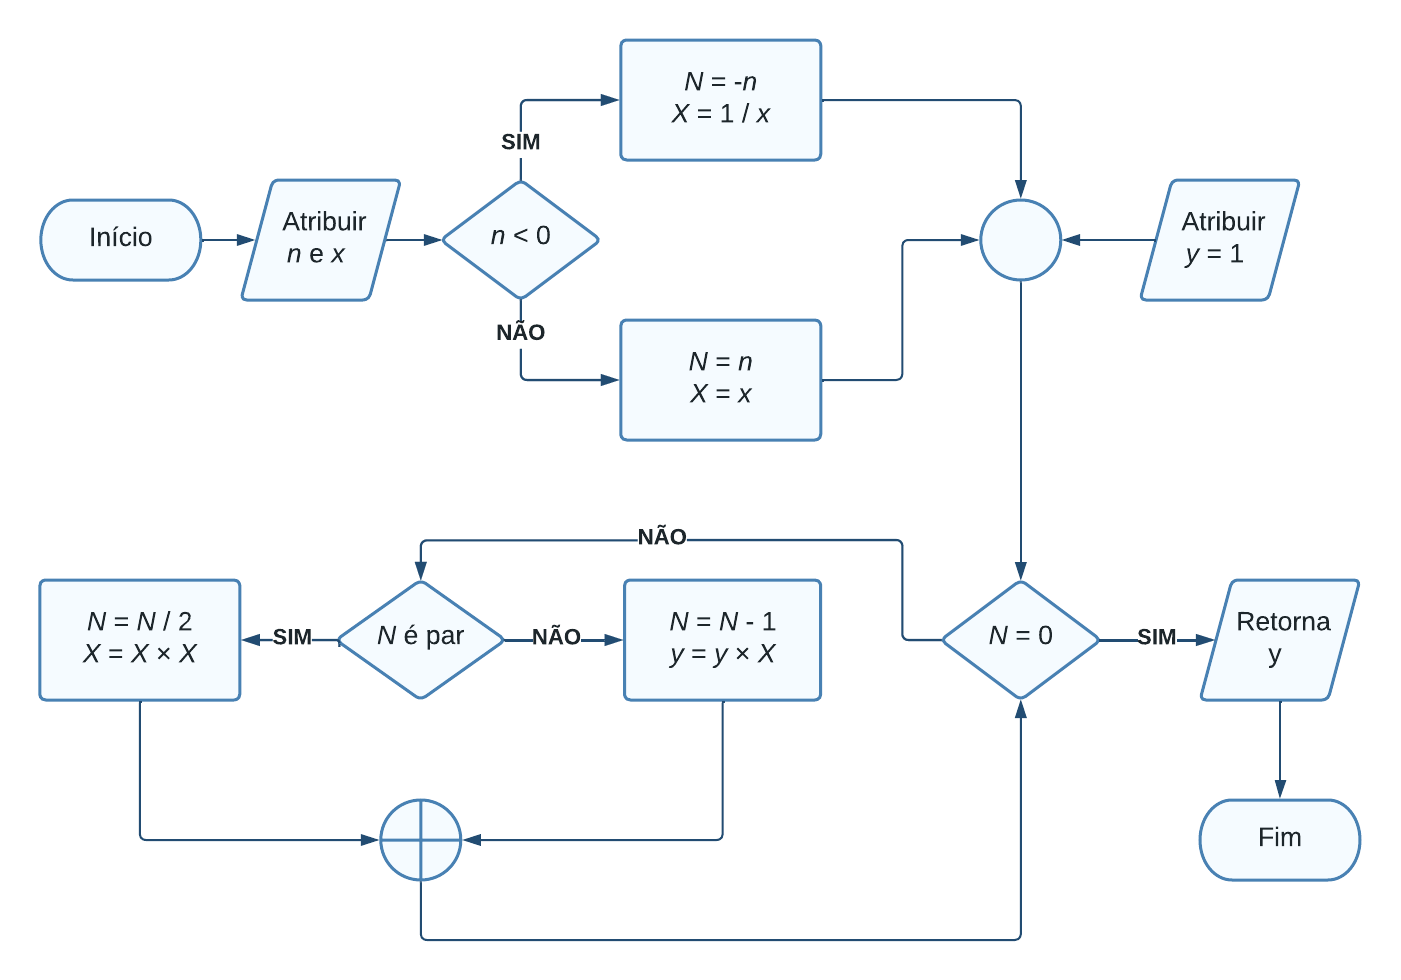
\includegraphics[width = \CaptionWidth]{fcht-ex-algorithms}
\SourceOrNote{autoria própria (\YearNum)}
\end{flowchart}

\subsection{Fotografias}%
\label{ssect:phot}

Um exemplo deste tipo de ilustração é apresentado na \Cref{phot:pg-campus}.

\begin{photograph}[!htbp]
\SetCaptionWidth{0.7\textwidth}
\caption[%
  Fachada do campus Ponta Grossa da UTFPR%
]{%
  Fachada do campus Ponta Grossa da \ifbool{MakeAcr}{\intl{UTFPR}}{UTFPR}%
}%
\label{phot:pg-campus}
\savebox0{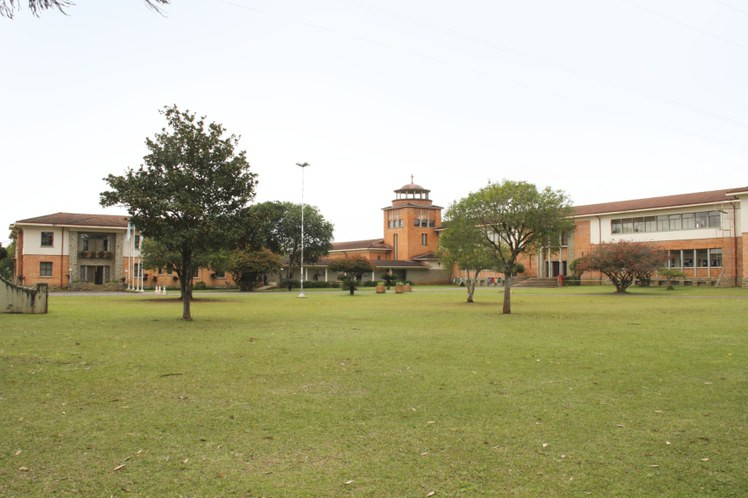
\includegraphics[width = \CaptionWidth]{phot-pg-campus}}
\usebox0%
\llap{%
  \raisebox{\ht0-\height}{%
    \href{https://www.utfpr.edu.br/campus/pontagrossa}{%
      
\includegraphics[height = 15mm]{phot-pg-campus-qr-code}%
    }%
  }%
}
\SourceOrNote{\textcite{UTFPR2018}}
\end{photograph}

Outro exemplo deste tipo de ilustração é apresentado na \Cref{phot:galunggung}.

\begin{photograph}[!htbp]
\SetCaptionWidth{0.7\textwidth}
\caption{Erupção vulcânica em 1982 do Galunggung (com descargas de raios) na Indonésia (foto de pesquisa realizada pelo Serviço Geológico dos Estados Unidos da América)}%
\label{phot:galunggung}
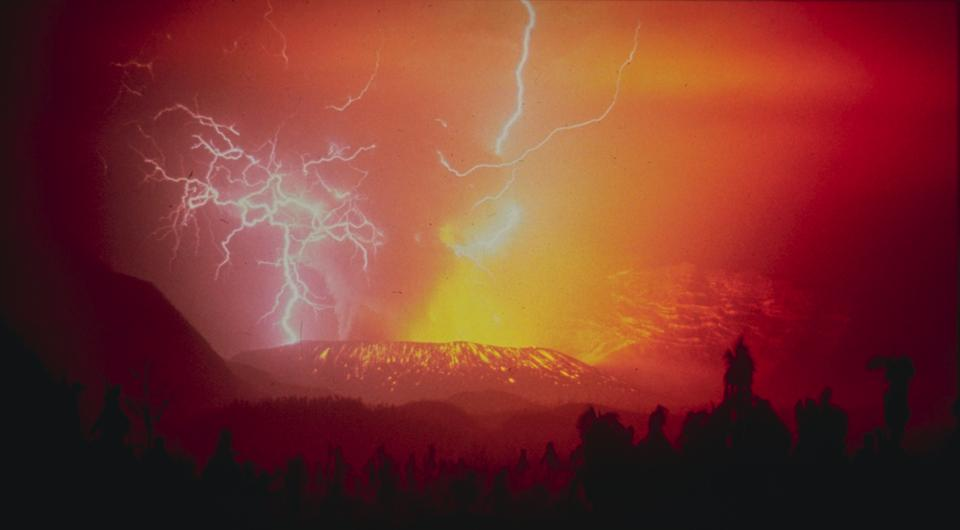
\includegraphics[width = \CaptionWidth]{phot-galunggung}%
\llap{%
  \href{https://en.wikipedia.org/wiki/Galunggung}{%
    
\includegraphics[height = 15mm]{phot-galunggung-qr-code}%
  }%
}
\SourceOrNote{\textcite{Hadian1982}}
\end{photograph}

Como mostrado nas \Cref{phot:pg-campus,phot:galunggung}, objetos flutuantes (ilustrações) podem adicionalmente receber um código de \ifbool{MakeAcr}{\intldescr{QR} (\intldescr+{QR} \textemdash\ \intl{QR})}{Resposta Rápida (\ENLang*{Quick Response} \textemdash\ QR)} contendo: \ifbool{MakeAcr}{\intldescr{URL} (\intldescr+{URL} \textemdash\ \intl{URL})}{Localizador Uniforme de Recursos (\ENLang*{Uniform Resource Locator} \textemdash\ URL)} ou informações complementares.

\subsection{Gráficos}%
\label{ssect:grph}

O ambiente \texttt{minipage} pode ser usado para inserir textos e outros elementos em caixas com tamanhos e posições controladas, conforme exemplos nos \Cref{grph:chi-beta,grph:t-x}, obtidos a partir dos arquivos-fonte \texttt{grph-chi-beta.tex} (\texttt{picture}) e \texttt{grph-t-x.tex} (\texttt{tikzpicture}) em \texttt{./Chapter-Example/Illustrations/}.

\begin{graph}[!htbp]
\begin{minipage}[t]{7cm}
\centering%
\SetCaptionWidth{\linewidth}
\caption{Primeiro exemplo de gráfico em ambiente \texttt{minipage}}%
\label{grph:chi-beta}
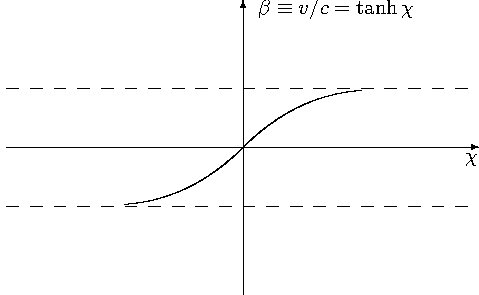
\includegraphics[width = \CaptionWidth]{grph-chi-beta}
\SourceOrNote{autoria própria (\YearNum)}
\end{minipage}
\hfill
\begin{minipage}[t]{8cm}
\centering%
\SetCaptionWidth{\linewidth}
\caption{Segundo exemplo de gráfico em ambiente \texttt{minipage}}%
\label{grph:t-x}
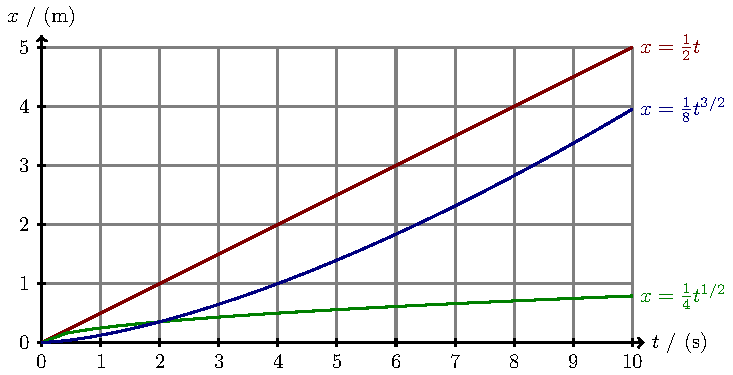
\includegraphics[width = \CaptionWidth]{grph-t-x}
\SourceOrNote{autoria própria (\YearNum)}
\end{minipage}
\end{graph}

Outro exemplo deste tipo de ilustração é apresentado no \Cref{grph:ex-gnuplot}.

\subsection{Quadros}%
\label{ssect:tfrm}

Quadros não devem ser chamados tabelas, visto que se diferenciam destas por apresentarem as laterais fechadas e o conteúdo não numérico, ou seja, são usados para dados qualitativos, predominantemente preenchidos com informações textuais (palavras).
Para quadros que ocupam mais de uma folha, não é necessária nenhuma sinalização.
Exemplos deste tipo de ilustração são apresentados nos \Cref{tfrm:acr-cmd,tfrm:sym-cmd,tfrm:math}.
